%%%%%%% DO NOT TOUCH IT! Or it might crash... dont come asking for support later ¯\_(ツ)_/¯. 
\documentclass[../../../../main.tex]{subfiles}
\graphicspath{ {\subfix{../../../../CTsettings/figures/}} {./figures/} {../figures/} {../../figures/}}
%%%%%%% DO NOT TOUCH IT! Or it might crash... dont come asking for support later ¯\_(ツ)_/¯. 


%%%%%%% DO NOT TOUCH IT! Or it might crash... dont come asking for support later ¯\_(ツ)_/¯. 
\begin{document}
\onlyinsubfile{
    \renewcommand{\onlyinsubfile}[1]{}
    \renewcommand{\notinsubfile}[1]{#1}

    \renewcommand{\onlyonmainfile}[1]{}
    \renewcommand{\onlyonpartfile}[1]{}
    \renewcommand{\onlyonchapterfile}[1]{}
    \renewcommand{\onlyonsectionfile}[1]{#1}

    \gdef\CTMcalibrefontpath{../../../../CTsettings/calibrefontfiles/}
    \setcalibrefont{\CTMcalibrefontpath}
    
    \fancypagestyle{plain}{\pagestyle{CTstylewithpage}}
    \pagestyle{CTstylewithpage}
}
%%%%%%% DO NOT TOUCH IT! Or it might crash... dont come asking for support later ¯\_(ツ)_/¯. 

\onlyonsectionfile{
}




\section{Monalisa Variant}


The \quotes{Monalisa} potato, as in Figure~\ref{fig:potato_monalisa}, scientifically known as Solanum tuberosum, is a popular and widely cultivated starchy tuber that belongs to the Solanaceae family. This unique variety is renowned for its distinctive appearance, which resembles the enigmatic smile of Leonardo da Vinci's famous painting, the "Mona Lisa." The Monalisa potato features a smooth, pale yellow to light brown skin with shallow eyes, making it visually distinct from other potato varieties.

Beneath its surface, the Monalisa potato reveals a creamy, pale yellow flesh that is high in starch content. This characteristic makes it ideal for various culinary applications, such as frying, baking, and boiling. Its starchy texture lends itself well to creating crispy and tender dishes, while also providing a neutral canvas for absorbing flavors and seasonings.

Due to its versatile nature and appealing appearance, the Monalisa potato has gained popularity in both home and commercial kitchens. It is often used to make classic dishes like French fries, potato wedges, mashed potatoes, and casseroles. Its ability to hold its shape during cooking and its ability to absorb flavors make it a favorite among chefs and home cooks alike.

Furthermore, the Monalisa potato is valued not only for its culinary attributes but also for its contribution to agriculture and global food security. Its widespread cultivation ensures a consistent supply of this staple crop, supporting diets around the world. Whether gracing a plate as crispy fries or mashed with butter and cream, the Monalisa potato remains a beloved ingredient cherished for its taste, versatility, and the whimsical resemblance it bears to the world of art.


\begin{figure}[!htbp]
    \centering
    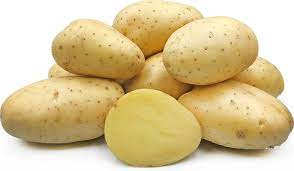
\includegraphics[width=0.5\textwidth]{Parts/PartExample/Chapters/potato_folder/figures/potato_monalisa.jpeg}
    \caption{Monalisa potato}
    \label{fig:potato_monalisa}
\end{figure}


\subsection{Monalisa Supreme Subvariant}
One notable subtype of the Monalisa potato variant is the "Monalisa Supreme." The Monalisa Supreme is a cultivated variation of the original Monalisa potato, distinguished by certain characteristics that set it apart within the culinary and agricultural spheres.

One of the standout features of the Monalisa Supreme is its enhanced culinary versatility. This subtype is often prized for its ability to maintain its shape and texture even after cooking, making it well-suited for dishes that require potatoes to hold their form. Whether used in salads, stews, or gratins, the Monalisa Supreme remains firm and appealing.

In addition to its culinary attributes, the Monalisa Supreme is also recognized for its improved resistance to certain pests and diseases. This resilience can be particularly advantageous for growers, as it reduces the need for excessive pesticide use and promotes more sustainable agricultural practices.

\begin{figure}[!htbp]
    \centering
    \begin{subfigure}{0.60\textwidth}
        \includegraphics[width=\textwidth]{./figures/potato_monalisa_superior.jpg}
        \caption{Subfigure Sightly Scaled}
    \end{subfigure}
    \hfill
    \begin{subfigure}{0.35\textwidth}
        \includegraphics[width=\textwidth]{./figures/potato_monalisa_superior.jpg}
        \caption{Subfigure Smaller}
    \end{subfigure}
    \caption{Monalisa Superior Potato}
\end{figure}



\begin{figure}[!htbp]
    \centering
    \begin{tikzpicture}
        % \node[rotate=45] {\includegraphics[width=0.5\textwidth]{Parts/PartExample/Chapters/potato_folder/figures/potato_monalisa_superior.jpg}}; %FULL PATH, avoid it! 
        \node[rotate=45] {\includegraphics[width=0.5\textwidth]{./figures/potato_monalisa_superior.jpg}};
    \end{tikzpicture}
    \caption{Rotated potato}
\end{figure}







The skin of the Monalisa Supreme is usually smooth and light brown, while its flesh retains the signature creamy and pale yellow hue common to Monalisa potatoes. Its shallow eyes and consistent appearance make it an appealing choice for both consumers and chefs, who value its uniformity when creating visually appealing dishes. \citep{yan_isotropic_2008}

Overall, the Monalisa Supreme subtype is a testament to ongoing efforts in potato breeding and cultivation \cite{du_vector-based_2017}. By enhancing both culinary qualities and disease resistance, this variant showcases the potential for crop improvement to meet the demands of modern agriculture and diverse culinary preferences.




\onlyonsectionfile{
\newpage
\important{Here I'll call a figure of parent folder. Lets see if it works. If not, in will only crash the section file.}

\begin{figure}[!htbp]
    \centering
    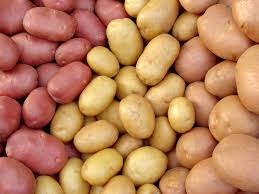
\includegraphics[width=0.5\textwidth]{../figures/potato_all.jpeg}
    \caption{Potato ALL}
    \label{fig:potato_monalisa2}
\end{figure}


}




%%%%%%% DO NOT TOUCH IT! Or it might crash... dont come asking for support later ¯\_(ツ)_/¯. 
\onlyonsectionfile{
\newpage
\section*{Bibliografia}
% \edef\mainjobname{\jobname}
% \edef\jobname{sectionmow\mainjobname}
\bibliographystyle{seg}
\bibliography{references.bib}
% \edef\jobname{\mainjobname}

}
%%%%%%% DO NOT TOUCH IT! Or it might crash... dont come asking for support later ¯\_(ツ)_/¯. 





\end{document}